\documentclass{article}
\usepackage{makeidx}
\usepackage{hyperref}
\usepackage{amsmath}
\usepackage{amssymb}
\usepackage{xcolor}
\usepackage{graphicx}

\title{Math Notes}
\author{Haotian Chen}
\date{}

\makeatletter
\renewcommand\paragraph{\@startsection{paragraph}{4}{\z@}%
                                     {-3.25ex\@plus -1ex \@minus -.2ex}%
                                     {1.5ex \@plus .2ex}%
                                     {\normalfont\normalsize\bfseries}}
\makeatletter

\hypersetup{
    colorlinks=true,
    linkcolor=blue,
    urlcolor=cyan,
}

\setcounter{tocdepth}{4}
\setcounter{secnumdepth}{4}

\makeindex



\begin{document}

\maketitle

\clearpage

\tableofcontents{}

\clearpage

\section{Statistics}

\subsection{Discrete Probability Distribution}

\noindent Let \(X\) be a random variable with a finite number of finite outcomes \( x_{1},  x_{2}, \ldots, x_{n}\) occurring with probabilities \(p_{1}, p_{2}, \ldots, p_{n}\) respectively. The expectation of \(X\) is defined as

\[\mu = E[X] = \sum_{i=1}^{n}x_{i} p_{i} = x_{1} p_{1} + x_{2} p_{2} + \cdots  + x_{n} p_{n}\]

\noindent The variance of \(X\) is

\[\sigma^{2} = Var(X) = \sum_{i=1}^{n}p_{i} \cdot (x_{i} - \mu)^{2}\]

\noindent For a collection of \(n\) equally likely values:

\[\mu = \frac {1}{n} \sum_{i=1}^{n} x_{i}\]
\[\sigma^{2} = \frac {1}{n} \sum_{i=1}^{n} (x_{i} - \mu)^{2}\]

\subsection{Continuous Probability Distribution}

\noindent If the random variable \(X\) has a probability density function \(f(x)\), and \(F(x)\) is the corresponding cumulative distribution function, then

\[\mu =\int_{\mathbb{R}} x f(x) dx = \int_{\mathbb{R}} x dF(x)\]
\[\sigma^{2} = \int_{\mathbb{R}}(x - \mu)^{2} f(x) dx\]

\subsubsection{Uniform Distribution}

\begin{center}
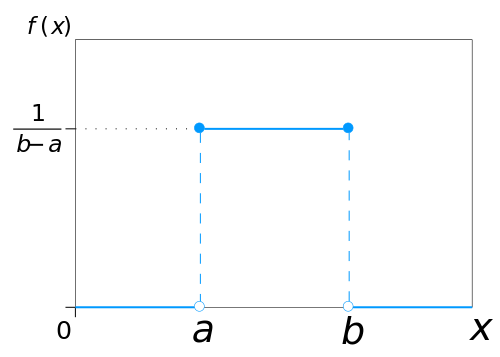
\includegraphics[scale=0.4]{./images/uniform_distribution_pdf.png}
\end{center}

\[
f(x) = 
\begin{cases}
\frac{1}{b-a} & \mathrm{for} \ a \leq x \leq b, \\
0 & \mathrm{for} \ x < a \ \mathrm{or} \ x > b
\end{cases}
\]
\[\mu = \tfrac{1}{2} (a + b)\]
\[\sigma^{2} = \tfrac{1}{12} (b - a)^{2}\]

\subsubsection{Normal Distribution}

\begin{center}
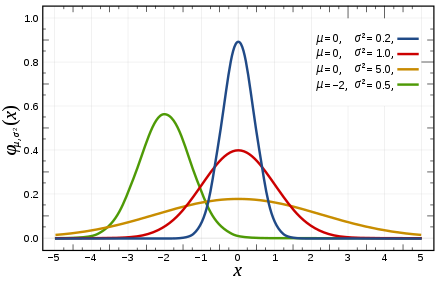
\includegraphics[scale=0.4]{./images/normal_distribution_pdf.png}
\end{center}

\[f(x) = \frac{1}{\sigma \sqrt{2\pi}} e^{-\frac{1}{2} (\frac{x - \mu}{\sigma })^{2}}\]

\printindex

\end{document}